This chapter builds on the previous to investigate the performance effects of different caching architectures and recovery mechanisms for NVRAM.
I look at NVRAM read and write performance concerns separately.
Additionally, I propose to include additional investigations into important aspects of the system such as bandwidth constraints and device lifetime (based on write endurance), outlined in Section~\ref{sec:OLTP_eval:Proposed}.

\section{NVRAM Reads}
\label{sec:OLTP_eval:Reads}

I first evaluate database performance with respect to NVRAM reads.
Many candidate NVRAM technologies exhibit greater read latency than DRAM, possibly requiring additional hardware or software caching.
I wish to determine, for a given NVRAM read latency, how much caching is necessary to prevent slowdown, and whether it is feasible to provide this capacity in a hardware-controlled cache (otherwise software caches must be used).

\subsection{NVRAM Caching Performance}
\label{sec:OLTP_eval:Reads:Performance}

\textbf{Traces.}
\begin{table*}
  \centering
  \begin{tabulary}{\textwidth}{L L L L L L L L L}
    \hline
    & \multicolumn{2}{c}{TATP} & \multicolumn{2}{c}{TPCB} & \multicolumn{2}{c}{TPCC} & \multicolumn{2}{c}{Average} \\
    & \% lines & lines/latch & \% lines & lines/latch & \% lines & lines/latch & \% lines & lines/latch \\
    \hline \hline
    Store & 10.57\% & 5.32 & 11.71\% & 6.05 & 15.47\% &  4.25 & 12.58\% & 5.20 \\
    Index & 89.43\% & 11.27 & 82.41\% & 12.19 & 81.18\% & 11.17 & 84.34\% & 11.54 \\
    Other & 0.00\% & 0.00 & 5.89\% & 7.16 & 3.36\% & 3.00 & 3.08\% & 3.39 \\
    Total & & 5.53 & & 8.47 & & 6.14 & & 6.71 \\
    \hline
  \end{tabulary}
  \caption{\textbf{NVRAM access characteristics.} ``\% lines" indicates the percentage breakdown of cache line accesses.  ``lines/latch" reports the average number of cache line accesses per page latch.  Indices represent the majority of accesses.}
  \label{table::AccessCharacteristics}
\end{table*}

The NVRAM read-performance model combines memory access trace analysis with the timing model to measure transaction throughput directly in Shore-MT.
Traces consist of memory accesses to the buffer cache, collected running Shore-MT with PIN for a single transaction thread for two minutes.
I assume concurrent threads exhibit similar access patterns.
In addition, I record all latch events (acquire and release) and latch page information (i.e., table id, store type -- index, store, or other).
I analyze traces at cache line (64 bytes) and page (8KB) granularity.

These traces provide insight into how Shore-MT accesses persistent data, summarized in Table~\ref{table::AccessCharacteristics}.
Index accesses represent the great majority of cache line accesses, averaging 84\% of accesses to NVRAM across workloads.
Any caching efforts should focus primarily on index pages and cache lines.
Note also that indices access a greater number of cache lines per page access than other page types (average 11.54 vs 5.20 per store and 3.39 per other page types), suggesting that uncached index page accesses have the potential to introduce greater delays. 

\textbf{Throughput.}
\begin{figure}
  \centering
  \subfigure[TATP]{\label{fig::ReadPerformance::TATP} 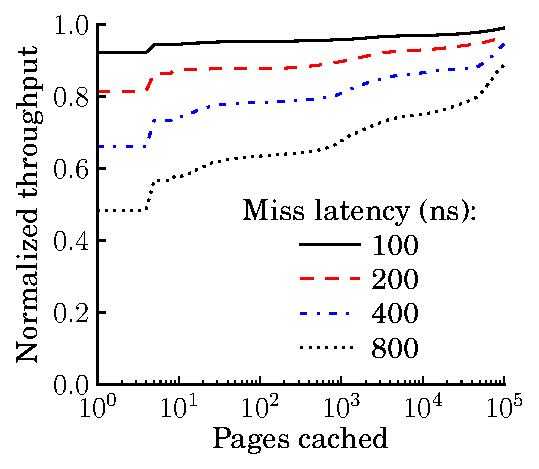
\includegraphics[width=.49\textwidth]{OLTP_eval/ReadPerformance_TATP.pdf}}
  \subfigure[TPCB]{\label{fig::ReadPerformance::TPCB}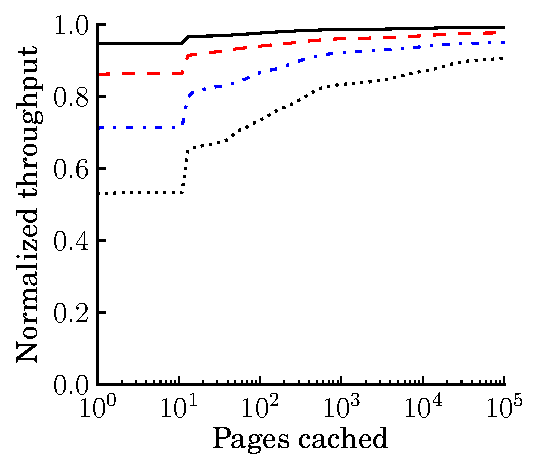
\includegraphics[width=.49\textwidth]{OLTP_eval/ReadPerformance_TPCB.pdf}}
  \subfigure[TPCC]{\label{fig::ReadPerformance::TPCC}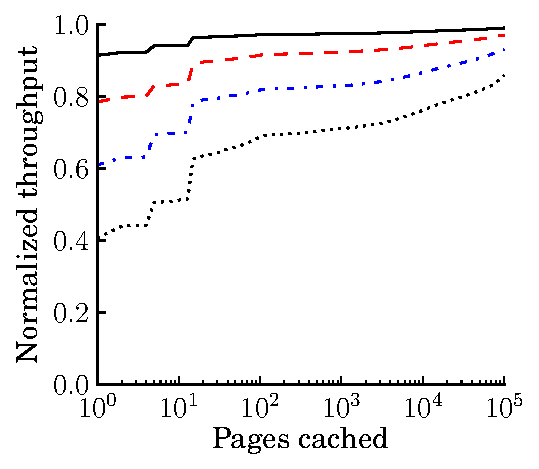
\includegraphics[width=.49\textwidth]{OLTP_eval/ReadPerformance_TPCC.pdf}}
%  \begin{subfigure}{0.32\textwidth}
%    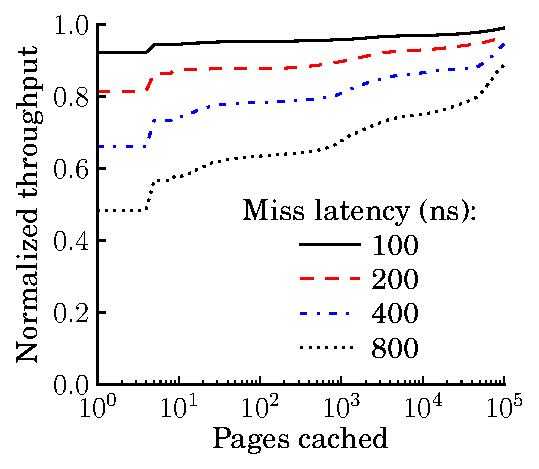
\includegraphics[width=\textwidth]{OLTP_eval/ReadPerformance_TATP.pdf}
%    \caption{TATP}
%    \label{fig::ReadPerformance::TATP}
%  \end{subfigure}
%  \begin{subfigure}{0.32\textwidth}
%    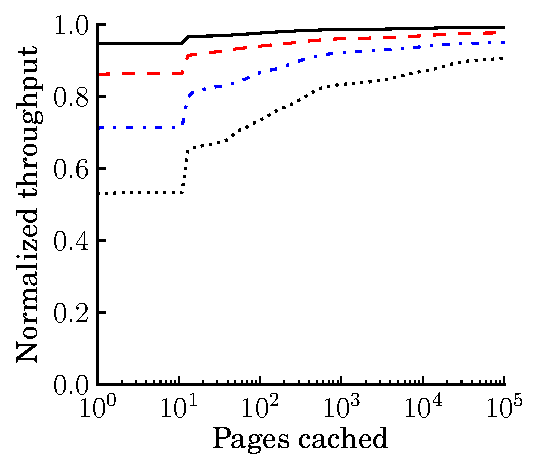
\includegraphics[width=\textwidth]{OLTP_eval/ReadPerformance_TPCB.pdf}
%    \caption{TPCB}
%    \label{fig::ReadPerformance::TPCB}
%  \end{subfigure}
%  \begin{subfigure}{0.32\textwidth}
%    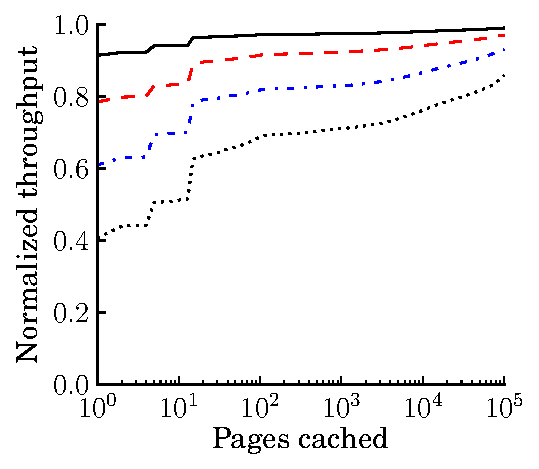
\includegraphics[width=\textwidth]{OLTP_eval/ReadPerformance_TPCC.pdf}
%    \caption{TPCC}
%    \label{fig::ReadPerformance::TPCC}
%  \end{subfigure}
  \caption{\textbf{Throughput vs NVRAM read latency.} 100ns miss latency suffers up to a 10\% slowdown over DRAM.  Higher miss latencies introduce large slowdowns, requiring caching.  Fortunately, even small caches effectively accelerate reads.}
  \label{fig::ReadPerformance}
\end{figure}

I create a timing model in Shore-MT from the previous memory traces.
Given traces, I perform cache analysis at page granularity, treating latches as page accesses and assuming a fully associative cache with a least-recently-used replacement policy (LRU).
Cache analysis produces an average page miss rate to each table.
I conservatively assume that every cache line access within an uncached page introduces an NVRAM stall, neglecting optimizations such as out-of-order execution and simultaneous multi-threading that might hide some NVRAM access stalls. 
The model assumes the test platform incurs a 50ns DRAM fetch latency, and adds additional latency to mimic NVRAM (for example, a 200ns NVRAM access adds 150ns delay per cache line).
I combine average page miss rate and average miss penalty (from lines/latch in table~\ref{table::AccessCharacteristics}) to compute the average delay incurred per latch event.
This delay is inserted at each page latch acquire in Shore-MT, using \InPlace, to produce a corresponding throughput.

Figure~\ref{fig::ReadPerformance} shows throughput achieved for the three workloads while varying the number of pages cached (horizontal axis) and NVRAM miss latency (various lines).
The vertical axis displays throughput normalized to DRAM-miss-latency's throughput (no additional delay inserted).
Without caching, throughput suffers as NVRAM miss latency increases, shown at the extreme left of each graph.
A 100ns miss latency consistently achieves at least 90\% of potential throughput.
However, an 800ns miss latency averages only 50\% of the potential throughput, clearly requiring caching.
Fortunately, caching proves remarkably effective for all workloads.
Each workload sees a spike of 10-20\% improvement for a cache size of just 20 pages.
As cache capacity further increases, each workload's throughput improves to varying degrees.
A cache capacity of 100,000 (or 819MB at 8KB pages) allows NVRAMs with 800ns miss latencies to achieve at least 80\% of the potential throughput.
While too large for on-chip caches, such a buffer might be possible as a hardware-managed DRAM cache \cite{QureshiSrinivasan09}.

\subsection{Analysis}
\label{sec:OLTP_eval:Reads:Analysis}
\begin{figure}
  \centering
  \subfigure[TATP]{\label{fig::Caching::TATP} 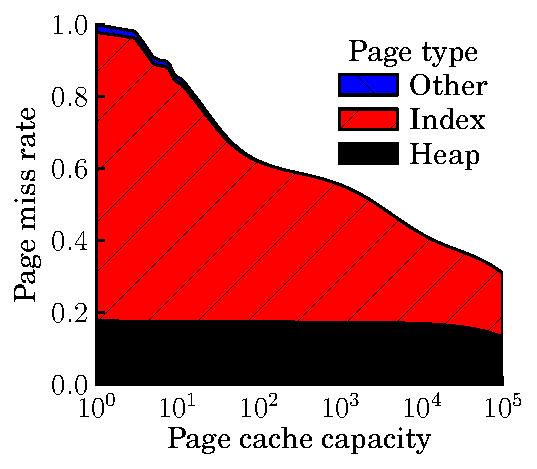
\includegraphics[width=.45\textwidth]{OLTP_eval/Caching_TATP.pdf}}
  \subfigure[TPCB]{\label{fig::Caching::TPCB}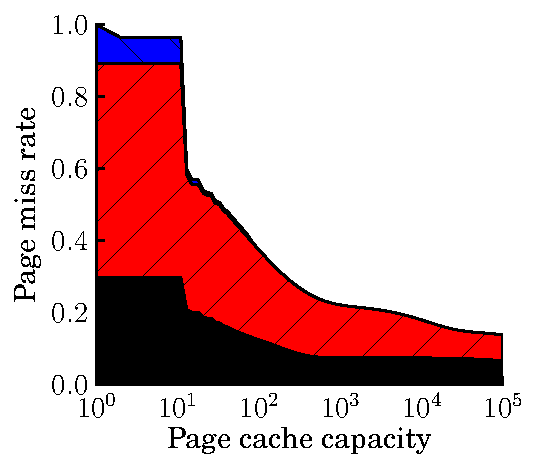
\includegraphics[width=.45\textwidth]{OLTP_eval/Caching_TPCB.pdf}}
  \subfigure[TPCC]{\label{fig::Caching::TPCC}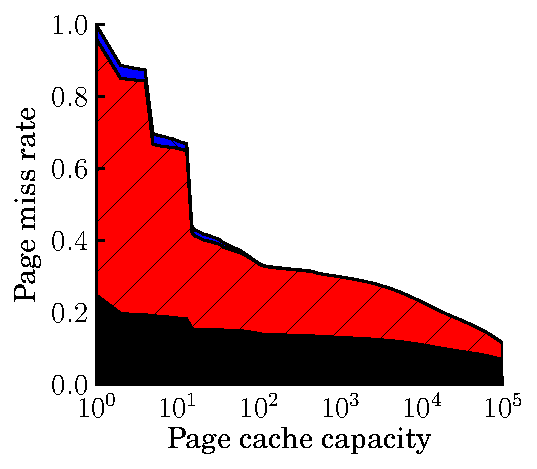
\includegraphics[width=.45\textwidth]{OLTP_eval/Caching_TPCC.pdf}}
  \caption{\textbf{Page caching effectiveness.} High level B+Tree pages and append-heavy store pages cache effectively.  Other pages cache as capacity approaches table size.}
  \label{fig::Caching}
\end{figure}

I have shown that modest cache sizes effectively hide NVRAM read stalls for these workloads, and further analyze caching behavior to reason about OLTP performance more generally.
Figure~\ref{fig::Caching} shows the page miss rate per page type (index, store, or other) as page cache capacity increases.
Each graph begins at 1.0 at the left -- all page accesses miss for a single page cache.
As cache capacity increases, workloads see their miss rates start to decrease between cache capacity of five and 20 pages.
TATP experiences a decrease in misses only in index pages, whereas TPCB and TPCC see a decrease across all page types.

While the behavior is specific to each workload, the results represent trends applicable to most databases and workloads, specifically, index accesses and append-heavy tables.
First, all workloads see a decrease in index page misses as soon as B+Tree roots (accessed on every traversal) successfully cache.
The hierarchical nature of B+Tree indices allows high levels of the tree to cache effectively for even a small cache capacity.
Additionally, TPCB and TPCC contain history tables to which data are primarily appended.
Transactions append to the same page as previous transactions, allowing such tables to cache effectively.
Similarly, extent map pages used for allocating new pages and locating pages to append into are frequently accessed and likely to cache.
The remaining tables' pages are accessed randomly and only cache as capacity approaches the size of each table.
In the case of TPCB and TPCC, each transaction touches a random tuple of successively larger tables (Branch, Teller, and Account for TPCB; Warehouse, District, Customer, etc. for TPCC).
This analysis suggests that various page types, notably index and append-heavy pages, cache effectively, accelerating throughput for high-latency NVRAM misses with small cache capacities.

\begin{table}
  \centering
  \begin{tabular}{l l}
    \hline
    Workload & Bandwidth (GB/s) \\
    \hline \hline
    TATP & 0.977 \\
    TPCB & 1.044 \\
    TPCC & 1.168 \\
    \hline
  \end{tabular}
  \caption{\textbf{Maximum required NVRAM read bandwidth.} Workloads require approximately 1 GB/s NVRAM read bandwith, well below technology limits.}
  \label{table::ReadBandwidth}
\end{table}

\textbf{Bandwidth.}
Finally, I briefly address NVRAM read bandwidth.
For a worst-case analysis, I assume no caching.
Given the average number of cache line accesses per page latch, the average number of page latches per transaction, and transaction throughput (taken from Section~\ref{sec:OLTP_eval:Persists}), I compute worst-case NVRAM read bandwidth for each workload, shown in Table~\ref{table::ReadBandwidth}~
The considered workloads require at most 1.168 GB/s (TPCC).
Since this is substantially lower than expected NVRAM bandwidth and caching reduces the required bandwidth further, I conclude that NVRAM read bandwidth for persistent data on OLTP is not a concern.

\subsection{Summary}
\label{sec:OLTP_eval:Reads:Summary}
NVRAM presents a new storage technology for which modern database systems have not been optimized.
Increased memory read latencies require new consideration for database caching systems.
I show that persistently stored data for OLTP can be cached effectively, even with limited cache capacity.
I expect future NVRAM software to leverage hardware caches, omitting software buffer caches.
Next, I turn to write performance for storage management on NVRAM devices.

\section{NVRAM Persist Synchronization}
\label{sec:OLTP_eval:Persists}

Whereas NVRAM reads benefit from caching, persists must always access the device.
Of particular insterest is the cost of ordering persists via persist barriers.
Several factors increase persist barrier latency, including ordering persists across distributed/NUMA memory architectures, long latency interconnects (e.g., PCIe-attached storage), and slow NVRAM MLC cell persists.
I consider the effect of persist barrier latency on transaction processing throughput to determine if and when new NVRAM technologies warrant redesigning recovery management.

Refer to Sections~\ref{sec:OLTP_design:Design} and~\ref{sec:OLTP_design:Methodology} for a more thorough description of recovery mechanisms and experimental setup.
All experiments throttle persist bandwidth to 1.5GB/s, which I believe to be conservative (possible with PCIe-attached flash).
Ideally, NVRAM will provide fast enough accesses to use \InPlace.
However, one would expect \InPlace's performance to suffer at large persist barrier latencies, requiring either \NVDisk or \GroupCommit to regain throughput.

\subsection{Persist Barrier Latency}
\label{sec:OLTP_eval:Persists:Performance}

\begin{figure*}
  \centering
  %\begin{subfigure}{0.32\textwidth}
  %  \includegraphics[width=\textwidth]{figures/pdfs/PersistLatencyThroughput/TATP.pdf}
  %  \caption{TATP}
  %  \label{fig::PersistLatencyThroughput::TATP}
  %\end{subfigure}
  %\begin{subfigure}{0.32\textwidth}
  %  \includegraphics[width=\textwidth]{figures/pdfs/PersistLatencyThroughput/TPCB.pdf}
  %  \caption{TPCB}
  %  \label{fig::PersistLatencyThroughput::TPCB}
  %\end{subfigure}
  %\begin{subfigure}{0.32\textwidth}
  %  \includegraphics[width=\textwidth]{figures/pdfs/PersistLatencyThroughput/TPCC.pdf}
  %  \caption{TPCC}
  %  \label{fig::PersistLatencyThroughput::TPCC}
  %\end{subfigure}
  \subfigure[TATP]{\label{fig::PersistLatencyThroughput::TATP} 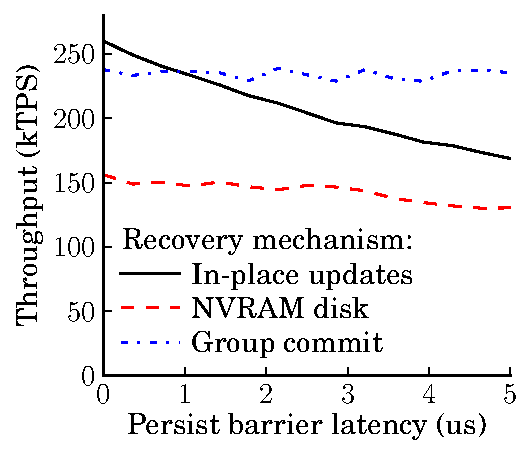
\includegraphics[width=.45\textwidth]{OLTP_eval/PersistLatencyThroughput_TATP.pdf}}
  \subfigure[TPCB]{\label{fig::PersistLatencyThroughput::TPCB}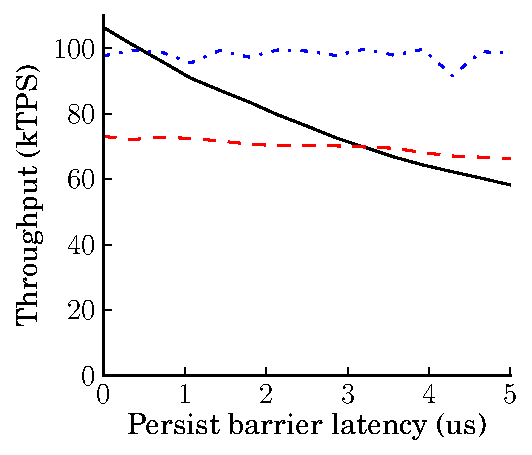
\includegraphics[width=.45\textwidth]{OLTP_eval/PersistLatencyThroughput_TPCB.pdf}}
  \subfigure[TPCC]{\label{fig::PersistLatencyThroughput::TPCC}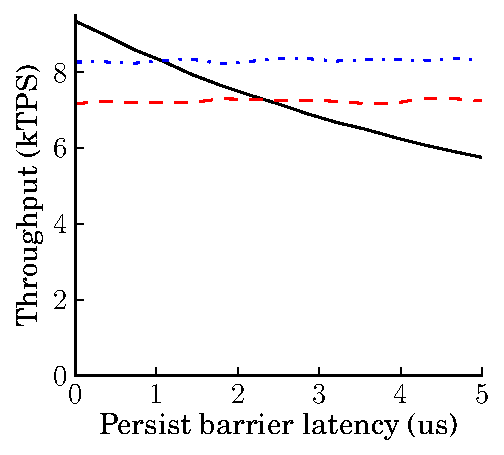
\includegraphics[width=.45\textwidth]{OLTP_eval/PersistLatencyThroughput_TPCC.pdf}}
  \caption{\textbf{Throughput vs persist barrier latency.} \InPlace performs best for zero-cost persist barriers, but throughput suffers as persist barrier latency increases.  \NVDisk and \GroupCommit are both insensitive to increasing persist barrier latency, with \GroupCommit offering higher throughput.}
  \label{fig::PersistLatencyThroughput}
\end{figure*}


Figure~\ref{fig::PersistLatencyThroughput} shows transaction throughput as persist barrier latency increases from 0\textmu s to 5\textmu s, the range believed to encompass realistic latencies for possible implementations of persist barriers and storage architectures.
A persist barrier latency of 0\textmu s (left edge) corresponds to no barrier/DRAM latency.
For such devices (e.g., battery-backed DRAM), \InPlace far out-paces \NVDisk, providing up to a 50\% throughput improvement.
The speedup stems from a combination of removing WAL overheads, removing contention between page flushers and transaction threads, and freeing up (a few) threads from log and page flushers to run additional transactions.
\InPlace also outperforms \GroupCommit, providing an average 10\% throughput improvement across workloads.

As persist barrier latency increases, each recovery mechanism reacts differently.
\InPlace, as expected, loses throughput.
\NVDisk and \GroupCommit, on the other hand, are both insensitive to persist barrier latency; their throughputs see only a small decrease as persist barrier latency increases.
TATP sees the largest throughput decrease for \NVDisk (14\% from 0\textmu s to 5\textmu s).
The decrease stems from \NVDisk's synchronous commits, requiring the log flusher thread to complete flushing before transactions commit.
During this time, transaction threads sit idle.
While both \NVDisk and \GroupCommit retain high throughput, there is a large gap between the two, with \GroupCommit providing up to a 50\% performance improvement over \NVDisk.
This difference, however, is workload dependent, with WAL imposing a greater bottleneck to TATP than to TPCB or TPCC.

Of particular interest are persist barrier latencies where lines intersect---the break-even points for determining the optimal recovery mechanism.
Whereas all workloads prefer \InPlace for a 0\textmu s persist barrier latency, \GroupCommit provides better throughput above 1\textmu s persist barrier latency.
When only considering \InPlace and \NVDisk the decision is less clear.
Over the range of persist barrier latencies TATP always prefers \InPlace to \NVDisk (the break-even latency is well above 5\textmu s).
TPCB and TPCC see the two mechanisms intersect near 3.5\textmu s and 2.5\textmu s, respectively, above which \NVDisk provides higher throughput.
TATP, unlike the other two workloads, only updates a single page per transaction.
Other overheads tend to dominate transaction time, resulting in a relatively shallow \InPlace curve.

These results suggest different conclusions across storage architectures.
NVRAM connected via the main memory bus will provide low latency persist barriers (less than 1\textmu s) and prefer \InPlace.
Other storage architectures, such as distributed storage, require greater delays to synchronize persists.
For such devices, \GroupCommit offers an alternative to \NVDisk that removes software overheads inherent in WAL while providing recovery.
However, \GroupCommit increases transaction latency.

\subsection{Transaction Latency}
\label{sec:OLTP_eval:Persists:XctLatency}

\begin{figure*}
  \centering
  %\begin{subfigure}{0.32\textwidth}
  %  \includegraphics[width=\textwidth]{figures/pdfs/XctLatency/TATP.pdf}
  %  \caption{TATP}
  %  \label{fig::XctLatency::TATP}
  %\end{subfigure}
  %\begin{subfigure}{0.32\textwidth}
  %  \includegraphics[width=\textwidth]{figures/pdfs/XctLatency/TPCB.pdf}
  %  \caption{TPCB}
  %  \label{fig::XctLatency::TPCB}
  %\end{subfigure}
  %\begin{subfigure}{0.32\textwidth}
  %  \includegraphics[width=\textwidth]{figures/pdfs/XctLatency/TPCC.pdf}
  %  \caption{TPCC}
  %  \label{fig::XctLatency::TPCC}
  %\end{subfigure}
  \subfigure[TATP -- Update Location]{\label{fig::XctLatency::TATP} 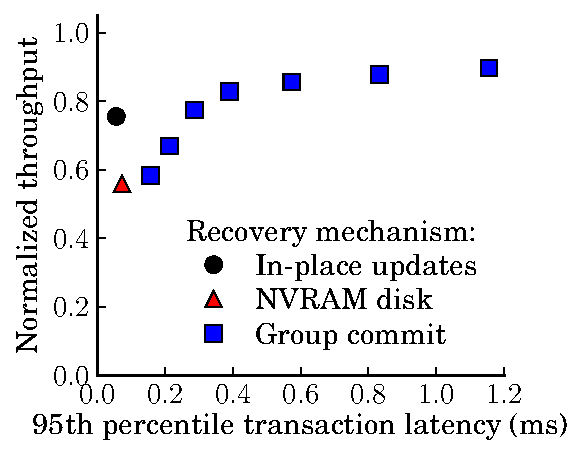
\includegraphics[width=.45\textwidth]{OLTP_eval/XctLatency_TATP.pdf}}
  \subfigure[TPCB]{\label{fig::XctLatency::TPCB}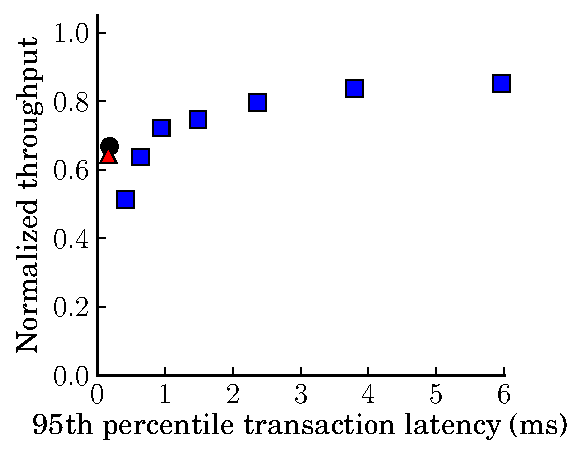
\includegraphics[width=.45\textwidth]{OLTP_eval/XctLatency_TPCB.pdf}}
  \subfigure[TPCC -- New Order]{\label{fig::XctLatency::TPCC}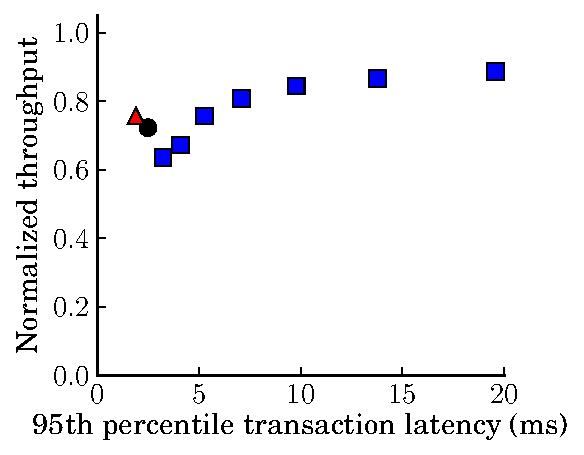
\includegraphics[width=.45\textwidth]{OLTP_eval/XctLatency_TPCC.pdf}}
  \caption{\textbf{95th percentile transaction latency.} All graphs are normalized to 0\textmu s persist barrier latency \InPlace throughput.  Experiments use 3\textmu s persist barrier latency.  \GroupCommit avoids high latency persist barriers by defering transaction commit, committing entire batches atomically.}
  \label{fig::XctLatency}
\end{figure*}


\GroupCommit improves transaction throughput by placing transactions into batches and committing all transactions in a batch atomically.
Doing so minimizes and limits the number of inserted persist barriers.
However, deferring transaction commit increases transaction latency, especially for the earliest transactions in each batch.
To achieve reasonable throughput, batches must be significantly longer than average transaction latency (such that batch execution time dominates batch quiesce and persist time).
The batch period acts as a knob for database administrators to trade off transaction latency and throughput.
I use this knob to measure the relationship between throughput and high-percentile transaction latency.

Figure~\ref{fig::XctLatency} shows throughput, normalized to \InPlace at 0\textmu s persist barrier latency.
The results consider a 3\textmu s persist barrier latency, where \GroupCommit provides a throughput improvement over other recovery mechanisms.
The different \GroupCommit points represent different batch periods, and I report the measured 95th percentile transaction latency for all recovery mechanisms.
I measure transaction latency from the time a transaction begins to the time its batch ends (Shore-MT does not model any pre-transaction queuing time).

The results illustrate that \GroupCommit is capable of providing equivalent throughput to the other recovery mechanisms with reasonable latency increases (no more than 5\texttimes).
Further, high-percentile transaction latencies fall well below the latency expectations of modern applications.
TPCC, the highest latency transaction, approaches optimal throughput with a 95th percentile transaction latency of 15ms---similar to latencies incurred by disk-backed databases.
For latency sensitive workloads, the batch period can be selected to precisely control latency, and \InPlace and \NVDisk remain alternatives.

\subsection{Summary}
\label{sec:OLTP_eval:Persists:Summary}
Persist barriers used to enforce persist order pose a new obstacle to providing recoverable storage management with NVRAM.
I show that, for memory bus-attached NVRAM devices, ensuring recovery using \InPlace is a viable strategy that provides high throughput and removes the overheads of WAL.
For interconnects and NVRAM technologies that incur larger persist barrier delays, \GroupCommit offers an alternative that yields high throughput and reasonable transaction latency.
\GroupCommit's batch period allows precise control over transaction latency for latency-critical applications.

\section{Proposed Work}
\label{sec:OLTP_eval:Proposed}

I propose to include two additional studies.
These studies were originally conducted for an earlier journal submission; the experimental system has changed substantially since then.

\textbf{Persist bandwidth.}
Different NVRAM storage architectures impose a variety of limitations on persist bandwidth (e.g., memory bus-attached NVRAM will allow greater throughput than PCIe-attached NVRAM).
I intend to study the persist bandwidth requirements for each recovery mechanism.

Recovery mechanisms display interesting behaviors with respect to bandwidth.
\NVDisk persists inefficiently with respect to the total number of store bytes updated; even a small page update requires large log entries.
However, the log persist makes effective use of cache lines (the granularity that data must transfer to the memory device).
Further, when increased recovery latency is allowable, bandwidth usage may be decreased by deferring page flushing, allowing writes to coalesce in pages.
The result is that \NVDisk makes reasonable use of bandwidth, and bandwidth constraints are unlikely to limit throughput.

\InPlace displays similar bandwidth usage to \NVDisk.
All page updates must persist to NVRAM, and these updates tend to use cache lines ineffectively (only a small portion of each cache line changes).
Also similarly to \NVDisk, \InPlace must maintain ARIES logs (although per-transaction and undo-only), requiring large persists.

\GroupCommit, while persisting the least amount of data, is the most sensitive to persist bandwidth constraints.
The total quantity of data is reduced by using physical logs -- logs copy data with little associated metadata.
Additionally, updates in each batch coalesce.
Only the first write to a given address produces undo, and only the final write to that address persists in-place.
Other versions of data during the batch do not persist.
The downside of \GroupCommit is that persists occur in bursts between batches.
No data persists while the batch executes.
Between batches however, all logs and store data persists, placing huge requirements on bandwidth.
I intend to include a quantitative study of this behavior.

\textbf{Device lifetime.}
NVRAM technologies, much like flash memory currently, will have limited write endurance; each cell may only be reliably written to a finite number of times.
Previous work suggests hardware techniques to evenly spread writes amongst cells.
The recovery mechanisms presented here each produce varying persist rates with different abilities to naturally spread persists across addresses/cells.
I intend to study expected device lifetime for each recovery mechanism, both assuming that persists to an address always persist to the same cell, and assuming hardware that evenly spreads persists across cells.

When persist-levelling hardware is not available \NVDisk manages to prolong lifetime the best of the three recovery mechanisms.
Centralized logs evenly persist to the entire log address space, which can be large.
Further, writes to individual pages can be bounded by limiting the page flush rate, although at the cost of recovery latency.
\InPlace performs worst in terms of device lifetime.
Updates to hot pages and addresses persist each distinct value, quickly wearing out hot cells.
\GroupCommit behaves reasonably, but is insufficient to provide lifetime guarantees for expected phase-change write endurance.
Persists coalesce within each batch.
This bounds persists to a single write per cell per batch.
However, as batches are short to lower transaction latency (on the order of 10ms) hot addresses continue to wear out quickly.

The story changes when hardware spreads persists across NVRAM cells.
The primary concern becomes the total number of persists.
While \GroupCommit outperforms \NVDisk and \InPlace in this regard, none of the recovery mechanisms pose a device lifetime concern.
Simply put, an insufficient amount of data persists to worry about device lifetime in the presence of hardware wear-leveling.

\section{Conclusion}
\label{sec:OLTP_eval:Conclusion}
New NVRAM technologies offer an alternative to disk that provides high performance while maintaining durable transaction semantics, yet existing database software is not optimized for such storage devices.
In this chapter, I evaluated recovery management to optimize for NVRAM read and persist characteristics.
I found that on-chip or other hardware caches prove sufficient to minimize NVRAM read stalls.
I also considered database performance in the presence of persist barrier delays.
As a drop-in replacement for disk, \NVDisk retains centralized logging overheads.
\InPlace reduces these overheads, but for large persist barrier latencies suffers from excessive synchronization stalls.
I proposed a new recovery mechanism, \GroupCommit, to minimize stalls due to persist synchronization while still removing centralized logging.
While \GroupCommit increases high-percentile transaction latency, latency is controllable and within modern application constraints.
